
%%%%%%%%%%%%%%%%%%%%%%%%%%%%%%%%%%%%%%%%%%%%%%%%%%%%%%%%%%%%%%%%%%%%%%%%%%%%%%%%
%%%%%%%%%%%%%%%%%%%%%%%%%%%%%%%%%%%%%%%%%%%%%%%%%%%%%%%%%%%%%%%%%%%%%%%%%%%%%%%%
% RESULTS %
%%%%%%%%%%%%%%%%%%%%%%%%%%%%%%%%%%%%%%%%%%%%%%%%%%%%%%%%%%%%%%%%%%%%%%%%%%%%%%%%

\cleardoublepage
\chapter{Results}
\label{chap:results}

This project is composed of different phases, as we have described throughout the dissertation. In this chapter, we will focus on analyzing the results obtained during the bad smells study and after the development of the assessment experiment.

\section{Analysis of bad smells}
\label{sec:results_analysis}

In the first place, we will detail the results of the entire study of bad smells, both the general and the statistical analysis. In each section we will try to answer the proposed research questions.  

\subsection{General analysis}
\label{subsec:results_general}

The general preliminary analysis of bad smells, as we described in the chapter~\ref{chap:implementation}, is focused on answering different questions related to the impact which bad smells have in the Scratch projects. In this section, we detail the results obtained from addressing our research questions using the previously described data set. 

\subsubsection{RQ1.To what extent are bad smells present in Scratch projects?}
\label{subsubsec:rq1_results}

As shown in Table~\ref{table:result_rq1}, bad smells can be found in almost all projects in our data set a - over 97\% of the projects have at least one bad smell. We expected a high share of projects having bad smells, but this result was a surprise for us, as the presence of bad smells is not only more frequent than expected, but almost general.

When we repeated the analysis with a larger set of projects, data set b, we found more moderate results. As we can also observe in Table~\ref{table:result_rq1}, around 64\% of the projects have at least one type of bad smell. Although it is still a very high percentage, this result was less alarming to us. These results are summarized in a more visual way in Figure~\ref{fig:rq1_result}.

\begin{table}
 \begin{center}
  \begin{tabular}{|c|c|c|c|}
    \hline
     & \textbf{Projects with at least} & \textbf{Projects with no} & \textbf{Total} \\ 
     & \textbf{one bad smell} & \textbf{bad smells} & \textbf{projects} \\ \hline
     \multirow{2}{*}{\textbf{Data set a}} & 97.97\% & 2.93\% & 100\% \\ 
     & 58,162 & 1,754 & 59,916 \\
     \hline
    \multirow{2}{*}{\textbf{Data set b}} & 64.24\% & 35.76\% & 100\% \\ 
     & 148,412 & 82,612 & 231,024 \\ \hline
  \end{tabular}
  \caption{Presence of bad smells in Scratch projects (RQ1).}
  \label{table:result_rq1}
 \end{center}
\end{table}

\begin{figure}
  \begin{subfigure}{.5\textwidth}
    \centering
    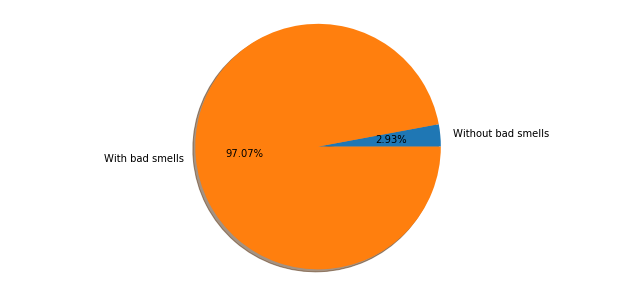
\includegraphics[width=9cm]{img/rq1_dataset_a.png}
    \caption{Data set a}
    \label{subfig:rq1_results_a}
  \end{subfigure}
  \begin{subfigure}{.5\textwidth}
    \centering
    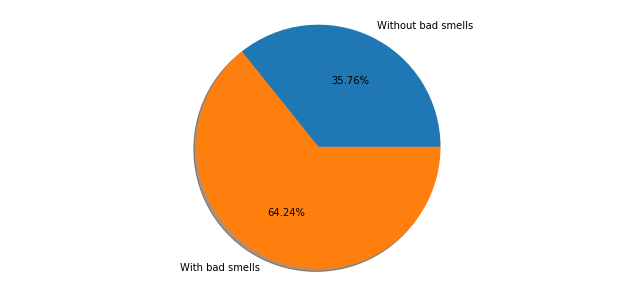
\includegraphics[width=9cm]{img/rq1_dataset_b.png}
    \caption{Data set b}
    \label{subfig:rq1_results_b}
  \end{subfigure}
  \caption{Presence of bad smells in Scratch projects (RQ1).}
  \label{fig:rq1_result}
\end{figure}  

\subsubsection{RQ2. Does the development of CT skills relate to a minor presence of bad smells?}
\label{subsub:rq2_results}

We have analyzed in more detail those projects that have and do not have bad smells. In particular, we want to see how the complexity of the projects is related to having a bad smell. We use the mastery required to create a project, as measured by Dr. Scratch, as a proxy for the complexity of the project.

The distribution of each set of projects is shown in Figure~\ref{fig:rq2_result}. In Figure~\ref{subfig:rq2_results_a} we can observe that more than 50\% of those projects with no bad smells have a total mastery of 0. In other words, these are skeleton projects without any content. The amount of projects with content and without any bad smell is therefore even lower than calculated in the previous research question. In addition, we see that projects with no bad smells are in the lower part of the complexity ladder.

In Figure~\ref{subfig:rq2_results_b} we can observe, as in the previous question, how the results are more moderate for data set b. In this second analysis, the mean value of the mastery obtained from the set of projects without any bad smells is higher, with 7 points on average (instead of 0 points). This result indicates that projects without bad smells are not mainly empty, although they are still very simple projects.

On the other hand, the results for the set of projects with bad smells are also softened. The distribution moves to the left in the graph and the average mastery decreases, although it continues in the higher part of the complexity ladder.

In summary, bad smells in Scratch can be found in almost all projects. Only a small set of projects with low complexity do not have them.

\begin{figure}
    \centering
    \begin{subfigure}{10cm}
    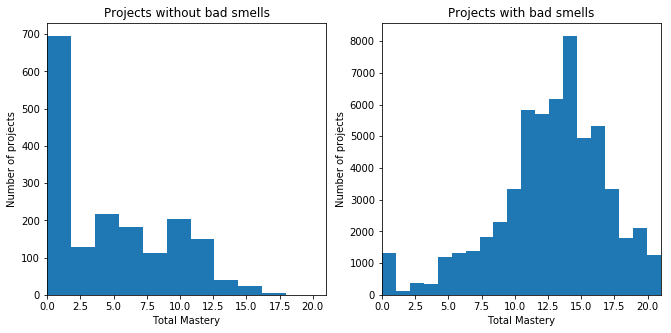
\includegraphics[width=10cm]{img/rq2_dataset_a.png}
    \caption{Data set a}
    \label{subfig:rq2_results_a}
  \end{subfigure}
  \begin{subfigure}{10cm}
    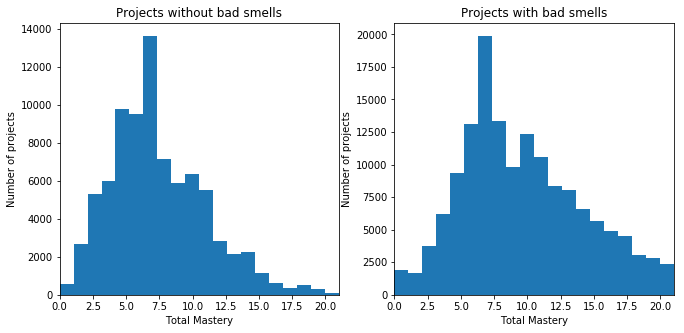
\includegraphics[width=10cm]{img/rq2_dataset_b.png}
    \caption{Data set b}
    \label{subfig:rq2_results_b}
  \end{subfigure}
    \caption{Distribution for projects without bad smells and with bad smells (RQ2).}
    \label{fig:rq2_result}
\end{figure}


\subsubsection{RQ3. Do projects with more blocks have a higher number of bad smells?}
\label{subsubsec:rq3_results}

One could argue that projects with more complexity (those with higher values of CT score in Dr. Scratch) usually have more blocks, and that the impact of a code smell there is lower than in less complex projects.

In other words, even if more complex projects have bad smells, their presence is mitigated by the fact that these are large projects. This would imply that achieving high values of CT development means to have less bad smells.

Figure~\ref{fig:rq3_result} visually shows the number of blocks for all projects for a given CT score (blue line) and the number of bad smells in those projects (red line). Both curves have been normalized to their maximum values.

In Figure~\ref{subfig:rq3_results_a}, we can observe how the two curves run almost in parallel. Up to 8 points they share the same ratio, then they share a ratio of around 0.5 up to 21 points, where the ratio is over 1.

Figure~\ref{subfig:rq3_results_b} not only represents the increase of bad smells with the number of blocks, but also a ratio over 1 in almost all the scores of CT (from 1 up to 20), when we normalize both variables. This result implies that bad smells are present in Scratch projects at all levels to a large extent. 

\begin{figure}
    \begin{subfigure}{.5\textwidth}
    \centering
    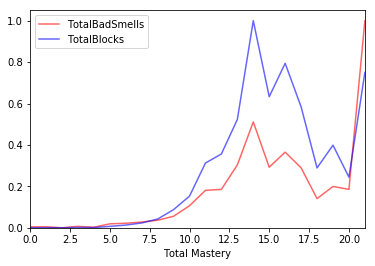
\includegraphics[width=8cm]{img/rq3_dataset_a.png}
    \caption{Data set a}
    \label{subfig:rq3_results_a}
  \end{subfigure}
  \begin{subfigure}{.5\textwidth}
    \centering
    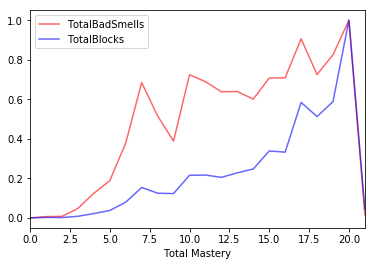
\includegraphics[width=8cm]{img/rq3_dataset_b.png}
    \caption{Data set b}
    \label{subfig:rq3_results_b}
  \end{subfigure}
    \caption{Relation between the total number of bad smells and the total number of blocks for each mastery level (RQ3).}
    \label{fig:rq3_result}
\end{figure}


\subsubsection{RQ4. Can we find a relation among specific bad smells?}
\label{subsubsec:rq4_results}

From Figure~\ref{subfig:rq4_results_a} (again, this graph is normalized), we can observe that the four different types of bad smells that we have studied have a similar distribution below the proficiency level. The presence of bad smells has a similar behavior for projects up to 17 points of mastery. Then, when the mastery is above 17 points, the behavior of each of them is different: While duplicated scripts and bad attribute initialization continue to slightly grow, the number of dead code blocks grows more abrupt way. However, the number of default names decreases considerably. This last trend may be because in projects with a high number of blocks and objects it is more difficult to program with the default names (Sprite 1, Sprite 2, etc) instead of personalizing them. 

In Figure~\ref{subfig:rq4_results_b} we have only data about three types of bad smells. For data set b, the information about attribute initialization was null, so we cannot represent it. 

Regarding the distribution of the other bad smells, all of them grow with a higher CT score, although default naming presents a most extreme curve. The main difference with Figure~\ref{subfig:rq4_results_a} can be observed for proficiency levels. When the mastery is above 17 points, all bad smells decrease considerably (for dead code this effect appears above 20 points). This trend would imply that proficiency profiles have greater awareness about the use of bad smells and they try to mitigate their use. 


\begin{figure}
    \begin{subfigure}{.5\textwidth}
    \centering
    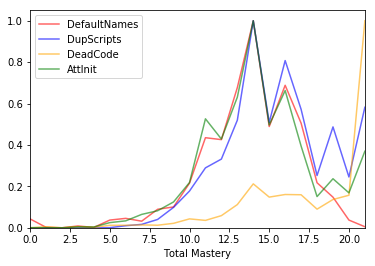
\includegraphics[width=8cm]{img/rq4_dataset_a.png}
    \caption{Data set a}
    \label{subfig:rq4_results_a}
  \end{subfigure}
  \begin{subfigure}{.5\textwidth}
    \centering
    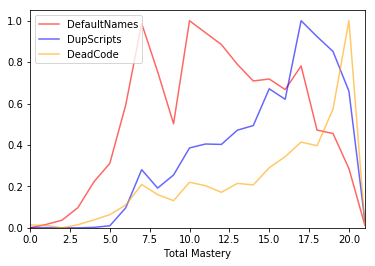
\includegraphics[width=8cm]{img/rq4_dataset_b.png}
    \caption{Data set b}
    \label{subfig:rq4_results_b}
  \end{subfigure}
    \caption{Evolution of the different types of bad smells with CT mastery (RQ4).}
    \label{fig:rq4_result}
\end{figure}


\subsubsection{RQ5. To which extent can bad smells be identified in each of the CT development phases?}
\label{subsubsec:rq5_results}

As already seen wit RQ3, the number of bad smells is higher when the total mastery increases. In Figure~\ref{fig:rq5_result}, we have represented the percentage of projects that have at least a specific type of bad smell for each level of CT proficiency. As we explained in the researching question RQ4, we do not have data about attribute initialization. For this reason, Figure~\ref{subfig:rq5_results_b} only shows three types of bad smells.

In both data set, the percentage of projects from users with basic level that have bad smells is much smaller than the percentage of projects that require a proficiency level. Although Figure~\ref{subfig:rq5_results_b} presents more moderate results than Figure~\ref{subfig:rq5_results_a}, both trends indicate that all bad smells have an incremental evolution with the increase of CT efficiency.

Therefore, it seems that bad smells appear in early phases and instead of disappearing with the development of more advanced CT skills, they become more prominent.

\begin{figure}
    \begin{subfigure}{.5\textwidth}
    \centering
    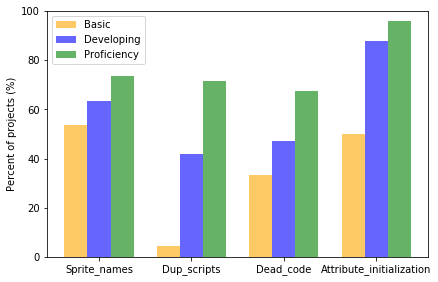
\includegraphics[width=8cm]{img/rq5_dataset_a.png}
    \caption{Data set a}
    \label{subfig:rq5_results_a}
  \end{subfigure}
  \begin{subfigure}{9cm}
    \centering
    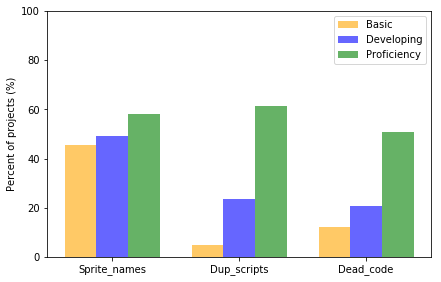
\includegraphics[width=8Cm]{img/rq5_dataset_b.png}
    \caption{Data set b}
    \label{subfig:rq5_results_b}
  \end{subfigure}
    \caption{Presence of bad smells for each proficiency level (RQ5).}
    \label{fig:rq5_result}
\end{figure}


\subsection{Statistical analysis}
\label{subsec:results_statistical}

The statistical analysis of bad smells is focused in a more specific study about the impact which bad smells have in our variable of interest, CT development. In this section, we describe the results obtained from the proposed research questions. 

\subsubsection{RQ1. Test \textit{t-student} with deciles}
\label{subsubsec:rq1_statistical_results}

In the first place, we analyzed the impact that bad smells have in the CT development in a general way.

\begin{itemize}
    \item[--] Population A: Projects in D9 which had less than 5 bad smells in D2 (N=168).
    \item[--] Population B: Projects in D9 which had more than 20 bad smells in D2 (N=95).
\end{itemize}

We found very interesting results. Except for \textit{dead code}, the results are very accurate. The \textit{p-value} of all of them is below 0.05, which implies that the differences between `Mean A' and `Mean B' are significant and not random. In other words, we found different evolution in both population and we could confirm that projects with a few bad smells in the beginning of a learning process, will have less bad smells in a period of time than projects which started with a higher value of bad smells. 

In addition, the \textit{size effect} presents a value about 0.5 or greater for all of them, except for the total number of bad smells. This may be caused by the noise introduced in the sum of all of them. These results are summarized in Table~\ref{table:rq1_statistical_results}.

However, we can observe in Table~\ref{table:rq1_statistical_results_mean} how the mean value of CT development in D2, measured with Dr. Scratch, is 9.57 for population A and 13.52 for population B. The different level of the CT skills at the beginning of a learning process could influence in the evolution of both groups. For this reason, we repeated the analysis for a more specific population with a more enclosed level of the CT skills.


\begin{table}
 \begin{center}
  \begin{tabular}{|c|c|c|c|c|}
    \hline
    \textbf{Bad Smell Type} & \textbf{Mean A} & \textbf{Mean B} & \textbf{p-value} & \textbf{Size effect} \\ \hline
    Default name & 1.45 & 8.56 & \textbf{1.105e-7} & -0.735 \\ \hline
    Duplicated code & 1.18 & 2.77 & \textbf{0.000200} & -0.494 \\ \hline
    Dead code & 3.45 & 33.52 & 0.054111 & -0.250 \\ \hline
    Attribute initialization & 4.23 & 12.68 & \textbf{5.576e-7} & -0.685 \\ \hline
    Total bad smells & 10.32 & 57.53 & \textbf{0.005191} & -0.367 \\ \hline
  \end{tabular}
  \caption{Results for the test \textit{t-student} with deciles (RQ1).}
  \label{table:rq1_statistical_results}
 \end{center}
\end{table}

\begin{table}
 \begin{center}
  \begin{tabular}{|c|c|c|}
    \hline
     & \textbf{Population A} & \textbf{Population B} \\ \hline
    \textbf{D2} & 9.57 & 13.52 \\ \hline
    \textbf{D9} & 13.64 & 14.73 \\ \hline
  \end{tabular}
  \caption{Mean value of the CT development scored with Dr. Scratch in D2 and D9 (RQ1).}
  \label{table:rq1_statistical_results_mean}
 \end{center}
\end{table}



\subsubsection{RQ2. Test \textit{t-student} with deciles for a given CT development}
\label{subsubsec:rq2_statistical_results}

As we described in the chapter~\ref{chap:implementation}, we repeated the analysis with projects whose CT level was included in the interval [7,12). 

\begin{itemize}
    \item[--] Population A: Projects in D9 which had less than 5 bad smells in D2 (N=62).
    \item[--] Population B: Projects in D9 which had more than 20 bad smells in D2 (N=21).
\end{itemize}

From this point, we obtained slightly worse results. Regarding \textit{duplicated code}, the \textit{p-value} obtained is greater than 0.05, so we cannot confirm that the differences between the mean value of bad smells in population A and population B are significant and not random.  The results are summarized in Table~\ref{table:rq2_statistical_results}.

On the other hand, the mean values of CT development in D2 are similar for each group, with a value of 9.45 points for population A and 9.81 points for population B, as we can observe in Table~\ref{table:rq2_statistical_results_mean}. However, the evolution of CT skills in D9 is not as we expected. Not only are very similar values, but they are slightly higher for population B. This result could imply that Dr. Scratch tool assess bad smells positively instead of penalizing them.

In order to verify this suppose, we repeated the analysis with other proposal and without deciles, as we described in RQ3.

\begin{table}
 \begin{center}
  \begin{tabular}{|c|c|c|c|c|}
    \hline
    \textbf{Bad Smell Type} & \textbf{Mean A} & \textbf{Mean B} & \textbf{p-value} & \textbf{Size effect} \\ \hline
    Default name & 1.34 & 7.90 & \textbf{0.001452} & -0.923 \\ \hline
    Duplicated code & 0.90 & 1.95 & 0.062411 & -0.494 \\ \hline
    Dead code & 3.16 & 10.38 & 0.136856 & -0.390 \\ \hline
    Attribute initialization & 3.97 & 11.86 & \textbf{0.020254} & -0.634 \\ \hline
    Total bad smells & 9.37 & 32.10 & \textbf{0.000208} & -1.107 \\ \hline
  \end{tabular}
  \caption{Results for the test \textit{t-student} with deciles for a given CT development (RQ2).}
  \label{table:rq2_statistical_results}
 \end{center}
\end{table}

\begin{table}
 \begin{center}
  \begin{tabular}{|c|c|c|}
    \hline
     & \textbf{Population A} & \textbf{Population B} \\ \hline
    \textbf{D2} & 9.45 & 9.81 \\ \hline
    \textbf{D9} & 12.90 & 13.14 \\ \hline
  \end{tabular}
  \caption{Mean value of the CT development scored with Dr. Scratch in D2 and D9 (RQ2).}
  \label{table:rq2_statistical_results_mean}
 \end{center}
\end{table}



\subsubsection{RQ3.1. Test \textit{t-student} without deciles for the total number of bad smells}
\label{subsubsec:RQ3_1_statistical_results}

The first analysis was developed in a general way for all bad smells.

\begin{itemize}
    \item[--] Population A: Projects in D1 which had less than 5 bad smells in D0 (N=129).
    \item[--] Population B: Projects in D1 which had more than 20 bad smells in D0 (N=11).
\end{itemize}


The results were not significant, since the \textit{p-value} and the \textit{size effect} were not relevant in any bad smell, as we can observe in Table~\ref{table:rq3_1_statistical_results}. We thought that these bad results were due to the noise introduced in the sum and the general analysis of each bad smell. For these reasons, we developed 
more specifically the test \textit{t-student} for each type of bad smell. 

On the other hand, nor did we find significant differences in the evaluation of the CT score by Dr. Scratch. As it is shown in Table~\ref{table:rq3_1_statistical_results_mean}, the mean value of CT development in D1 is so close for population A and population B. Therefore, we could not confirm the suppose found in RQ2. 



\begin{table}
 \begin{center}
  \begin{tabular}{|c|c|c|c|c|}
    \hline
    \textbf{Bad Smell Type} & \textbf{Mean A} & \textbf{Mean B} & \textbf{p-value} & \textbf{Size effect} \\ \hline
    Default name & 3.02 & 1.45 & 0.097957 & 0.531 \\ \hline
    Duplicated code & 1.44 & 1.23 & 0.662653 & 0.139 \\ \hline
    Dead code & 4.99 & 16.18 & 0.209101 & -0.421 \\ \hline
    Attribute initialization & 5.42 & 8.88 & 0.499307 & -0.220 \\ \hline
    Total bad smells & 14.88 & 27.73 & 0.191010 & -0.438 \\ \hline
  \end{tabular}
  \caption{Results for the test \textit{t-student} without deciles for the total number of bad smells (RQ3.1).}
  \label{table:rq3_1_statistical_results}
 \end{center}
\end{table}

\begin{table}
 \begin{center}
  \begin{tabular}{|c|c|c|}
    \hline
     & \textbf{Population A} & \textbf{Population B} \\ \hline
    \textbf{D0} & 7.0 & 7.0 \\ \hline
    \textbf{D1} & 13.15 & 13.45 \\ \hline
  \end{tabular}
  \caption{Mean value of the CT development scored with Dr. Scratch in D0 and D1 (RQ3.1).}
  \label{table:rq3_1_statistical_results_mean}
 \end{center}
\end{table}



\subsubsection{RQ3.2. Test \textit{t-student} without deciles for default naming}
\label{subsubsec:RQ3_2_statistical_results}

In the first place, we realized that the \textit{median} as measure variable was more relevant than the \textit{mean}. For this reason, since this analysis, we used \textit{median} instead of \textit{mean}. 

In the second place, we found very interesting results. The \textit{p-value} for all the study cases was below 0.05, which indicates that the differences between population A and population B are relevant. In addition, the \textit{size effect} had also a good value, around 0.500 for case 1 and greater for the rest of them. These results are summarized in Table~\ref{table:rq3_2_statistical_results}. 

However, we confirmed our suppose in RQ2. As we can observe in Table~\ref{table:rq3_2_statistical_results_median}, the CT score measured by Dr. Scratch in D1 increases with each case -that is, with the increase of the percent of default names-, due to the higher number of blocks and sprites. This result means that Dr. Scratch does not take into account the increase in default names, but only the increase in the number of blocks and sprites.

\begin{table}
 \begin{center}
  \begin{tabular}{|c|c|c|c|c|}
    \hline
    \textbf{Default Name} & \textbf{Median A} & \textbf{Median B} & \textbf{p-value} & \textbf{Size effect} \\ \hline
    Case 1 & 0.0 & 3.0 & \textbf{0.001889} & -0.486 \\ \hline
    Case 2 & 0.0 & 6.0 & \textbf{0.004488} & -0.617 \\ \hline
    Case 3 & 0.0 & 6.0 & \textbf{0.000217} & -0.934 \\ \hline
    Case 4 & 0.0 & 6.0 & \textbf{0.000469} & -0.919 \\ \hline
  \end{tabular}
  \caption{Results for the test \textit{t-student} without deciles for default naming (RQ3.2).}
  \label{table:rq3_2_statistical_results}
 \end{center}
\end{table}


\begin{table}
 \begin{center}
  \begin{tabular}{|c|c|c|c|c|c|c|c|}
    \cline{3-8}
     \multicolumn{2}{c}{} & 
     \multicolumn{2}{|c|}{\textbf{Median CT score}} & \multicolumn{2}{|c|}{\textbf{Median blocks}} & \multicolumn{2}{|c|}{\textbf{Median sprites}} \\ \cline{3-8}
     \multicolumn{2}{c|}{} & 
     A & B & A & B & A & B \\ \hline
     \multirow{4}{*}{\textbf{D0}}
     & Case 1 & 7.0 & 7.0 & 19.0 & 14.0 & 2.0 & 3.0 \\
     & Case 2 & 7.0 & 7.0 & 19.0 & 11.5 & 2.0 & 2.5 \\
     & Case 3 & 7.0 & 7.0 & 19.0 & 11.5 & 2.0 & 2.0 \\
     & Case 4 & 7.0 & 7.0 & 19.0 & 12.0 & 2.0 & 2.0 \\ \hline
     \multirow{4}{*}{\textbf{D1}}
     & Case 1 & 12.0 & 13.5 & 116.0 & 143.0 & 7.0 & 9.0 \\
     & Case 2 & 12.0 & 14.0 & 116.0 & 180.5 & 7.0 & 9.5 \\
     & Case 3 & 12.0 & 14.0 & 116.0 & 180.5 & 7.0 & 9.5 \\
     & Case 4 & 12.0 & 14.0 & 116.0 & 187.5 & 7.0 & 9.5 \\ \hline
  \end{tabular}
  \caption{Median value of CT development scored with Dr. Scratch, blocks and sprites for default naming (RQ3.2).}
  \label{table:rq3_2_statistical_results_median}
 \end{center}
\end{table}


\subsubsection{RQ3.3. Test \textit{t-student} without deciles for duplicated code}
\label{subsubsec:RQ3_3_statistical_results}

The results of this analysis are not as relevant as the results for default naming, as we can observe in Table~\ref{table:rq3_3_statistical_results}. The \textit{p-value} and the \textit{size effect} do not indicate significant results and we cannot confirm that the presence of duplicated code in the beginning of a learning process impacts in the CT development. 

However, our suppose can be confirmed again. In Table~\ref{table:rq3_3_statistical_results_median} we can observe how the CT score for population B in D1 is higher than the CT score for population A. This result indicates that Dr. Scratch is assessing positively the presence of duplicated code by the simple fact that the project has a larger number of blocks.

\begin{table}
 \begin{center}
  \begin{tabular}{|c|c|c|c|c|}
    \hline
    \textbf{Duplicated Code} & \textbf{Median A} & \textbf{Median B} & \textbf{p-value} & \textbf{Size effect} \\ \hline
    Case 1 & 0.0 & 1.0 & 0.217311 & -0.455 \\ \hline
  \end{tabular}
  \caption{Results for the test \textit{t-student} without deciles for duplicated code (RQ3.3).}
  \label{table:rq3_3_statistical_results}
 \end{center}
\end{table}

\begin{table}
 \begin{center}
  \begin{tabular}{|c|c|c|c|c|}
    \cline{2-5}
     \multicolumn{1}{c}{} & 
     \multicolumn{2}{|c|}{\textbf{Median CT score}} & \multicolumn{2}{|c|}{\textbf{Median blocks}} \\
     \cline{2-5}
     \multicolumn{1}{c|}{} & A & B & A & B \\ \hline
     \textbf{D0} & 7.0 & 7.0 & 17.0 & 39.0 \\ \hline
     \textbf{D1} & 13.0 & 14.0 & 131.0 & 218.0 \\ \hline
  \end{tabular}
  \caption{Median value of blocks and CT development scored with Dr. Scratch for duplicated code (RQ3.3).}
  \label{table:rq3_3_statistical_results_median}
 \end{center}
\end{table}



\subsubsection{RQ3.4. Test \textit{t-student} without deciles for dead code}
\label{subsubsec:RQ3_4_statistical_results}

The results of the \textit{t-student} test for dead code are very similar to the analysis of duplicated code. The \textit{p-value} and the \textit{size effect} have not significant values. Therefore, nor can we confirm that the presence of dead code in the beginning of a learning process has an impact in the CT development. These results are summarized in Table~\ref{table:rq3_4_statistical_results}.

Regarding the assessment of Dr. Scratch, we found the same effect in this analysis. As we can observe in Table~\ref{table:rq3_4_statistical_results_median}, the CT score in D1 is higher for population A than the CT score for population B. However, this result is not due to the presence or not of dead code, but to the larger number of blocks in population A. When the number of blocks in population B decreases -maybe because of the elimination of dead code- the value of the CT development also decreases, instead of receiving a positive recognition.

\begin{table}
 \begin{center}
  \begin{tabular}{|c|c|c|c|c|}
    \hline
    \textbf{Dead Code} & \textbf{Median A} & \textbf{Median B} & \textbf{p-value} & \textbf{Size effect} \\ \hline
    Case 1 & 0.0 & 5.0 & 0.096581 & -0.250 \\ \hline
    Case 2 & 0.0 & 6.0 & 0.080498 & -0.289 \\ \hline
    Case 3 & 0.0 & 5.0 & 0.131713 & -0.325 \\ \hline
  \end{tabular}
  \caption{Results for the test \textit{t-student} without deciles for dead code (RQ3.4).}
  \label{table:rq3_4_statistical_results}
 \end{center}
\end{table}


\begin{table}
 \begin{center}
  \begin{tabular}{|c|c|c|c|c|c|}
    \cline{3-6}
     \multicolumn{2}{c}{} & 
     \multicolumn{2}{|c|}{\textbf{Median CT score}} & \multicolumn{2}{|c|}{\textbf{Median blocks}} \\ 
     \cline{3-6}
     \multicolumn{2}{c|}{} & A & B & A & B \\ \hline
     \multirow{3}{*}{\textbf{D0}}
     & Case 1 & 7.0 & 7.0 & 13.5 & 21.0 \\
     & Case 2 & 7.0 & 7.0 & 13.5 & 21.0 \\
     & Case 3 & 7.0 & 7.0 & 13.5 & 22.5 \\ \hline
     \multirow{3}{*}{\textbf{D1}}
     & Case 1 & 14.0 & 8.0 & 198.5 & 58.0 \\
     & Case 2 & 14.0 & 7.0 & 198.5 & 31.0 \\
     & Case 3 & 14.0 & 8.5 & 198.5 & 71.5 \\ \hline
  \end{tabular}
  \caption{Median value of blocks and CT development scored with Dr. Scratch for dead code (RQ3.4).}
  \label{table:rq3_4_statistical_results_median}
 \end{center}
\end{table}



\subsubsection{RQ3.5. Test \textit{t-student} without deciles for attribute initialization}
\label{subsubsec:RQ3_5_statistical_results}

Lastly, we obtained the same effects on the results of the analysis with attribute initialization. In Table~\ref{table:rq3_5_statistical_results} we can observe that the values of \textit{p-value} and \textit{size effect} are not relevant. Therefore, we cannot confirm that a worse initialization of attributes has an impact in the CT development process. 

In addition, we can observe slightly the trend of the previous analyzes in Table~\ref{table:rq3_5_statistical_results_median}. The value of CT scored with Dr. Scratch is a little greater, from 14.0 to 14.5 points, when the number of blocks increases significantly, from 175.5 to 328.5.

\begin{table}
 \begin{center}
  \begin{tabular}{|c|c|c|c|c|}
    \hline
    \textbf{Attribute Initialization} & \textbf{Median A} & \textbf{Median B} & \textbf{p-value} & \textbf{Size effect} \\ \hline
    Case 1 & 3.0 & 6.0 & 0.101538 & -0.499 \\ \hline
    Case 2 & 3.0 & 10.0 & 0.092452 & -0.873 \\ \hline
  \end{tabular}
  \caption{Results for the test \textit{t-student} without deciles for attribute initialization (RQ3.5).}
  \label{table:rq3_5_statistical_results}
 \end{center}
\end{table}

\begin{table}
 \begin{center}
  \begin{tabular}{|c|c|c|c|c|c|}
    \cline{3-6}
     \multicolumn{2}{c}{} & 
     \multicolumn{2}{|c|}{\textbf{Median CT score}} & \multicolumn{2}{|c|}{\textbf{Median blocks}} \\ 
     \cline{3-6}
     \multicolumn{2}{c|}{} & A & B & A & B \\ \hline
     \multirow{2}{*}{\textbf{D0}}
     & Case 1 & 7.0 & 7.0 & 14.0 & 9.0 \\
     & Case 2 & 7.0 & 7.0 & 10.0 & 7.0 \\ \hline
     \multirow{2}{*}{\textbf{D1}}
     & Case 1 & 14.0 & 14.0 & 175.5 & 189.0 \\
     & Case 2 & 14.0 & 14.5 & 175.5 & 328.5 \\ \hline
  \end{tabular}
  \caption{Median value of blocks and CT development scored with Dr. Scratch for attribute initialization (RQ3.5).}
  \label{table:rq3_5_statistical_results_median}
 \end{center}
\end{table}

\hfill

In summary, with a more specific analysis with the \textit{t-student} test and more controlled populations, we cannot affirm that the presence of bad smells has an impact in the development of the CT skills in a learning process. However, we have found an alarming fact that should be analyzed in more detail: not only the Dr. Scratch tool does not assess negatively the presence of bad smells in the Scratch projects, but gives them more punctuation if they are present in projects with a larger number of blocks.

\section{Assessment experiment}
\label{sec:results_experiment}

Finally, we will show the results collected from the assessment experiment developed. 
